\section{The Data}
\label{seq:the data}
Each model is built on a set of data and for our models this is no different. The data is provided by Picnic B.V. Picnic is an online supermarket in the Netherlands, Germany and in France. However since the operations in France are still in an earlier face, we will only focus on the Netherlands and Germany in this Thesis. Picnic maintains a high quality Data Warehouse, but since the company is still very young, only the data starting from  from 01-10-2020 until 11-11-2022 can be used. This has to do with the Picnic data being reliable from 01-10-2020 onward because at this date the Picnic customer service department fully switched to a Salesforce system for all the customer success data. This is important for the data as the Salesforce system allows for more and better quality data collection.\\

There are two databases which have the same structure. One database with data from the Netherlands and one database with data from Germany. The data from the two countries is quite different as the operations in the Netherlands are more mature. Picnic started in the Netherlands in 2015 in Amersfoort and Picnic started in 2018 in Germany in North Rhine-Westphalia.

\subsection{Data Description}
The Picnic data is enriched with public data sources for School vacations and national holidays. This leaves us with a data set consisting of both categorical data and continuous data. The features we will use (except in the Local Level, Regression and ARIMA models) are: The first and seventh lag of the number of cases, the Number of deliveries at a certain day, the average countrywide weather temperature in Celsius, the average countrywide UV index, how many school regions have school vacation, if the day is a national holiday and lastly a unique constant for every day of the week.\\

The weather data will be different depending on the forecast horizon. This data is provided by Weather Source. For the closest horizons, we will use the weather forecasts provided by weather source. As weather forecasts are very unreliable in the further future \citep{Scher2018PredictingLearning}, the 10 year average for temperature and UV index will be used in the forecasts horizons that are further into the future.\\

The data from the school vacations comes from the Dutch Rijksoverheid website where an API exists that is used. For the German school vacations data is used from the ferien-api by Paul Brejla \citep{BrejlaDeutscheFerientermine}. For both countries the national holidays are acquired by the PyPi holidays package.\\

\begin{table}[]
    \centering
    \begin{tabular}{|c|c c c|}\hline
        Netherlands & Variance & Standard Deviation & Mean\\
        \hline
        Junior & 114222.558 & 337.968 & 1744.184\\
        Medior & 37820.469 & 194.475 & 690.138\\
        Senior & 33143.628 & 182.054 & 756.292\\
        Webcare & 189.83 & 13.778 & 19.801\\
        Assortment & 133249.88 & 365.034 & 1402.608\\
        \hline
        Germany & Variance & Standard Deviation & Mean\\
        \hline
        Junior & 199651.476 & 446.824 & 1037.731\\
        Medior & 18059.271 & 134.385 & 402.948\\
        Senior & 10507.892 & 102.508 & 190.057\\
        Webcare & 4.205 & 2.051 & 3.329\\
        Assortment & 23398.984 & 152.967 & 561.868\\\hline
    \end{tabular}
    \caption{Mean, Standard deviation and Variance and average time spend of the cases per skill level}
    \label{tab:mean_var}
\end{table}

\begin{table}[]
    \centering
    \begin{tabular}{|c|c c c|}\hline
        Netherlands & Variance & Standard Deviation & Mean\\
        \hline
        Total Deliveries & 36483231 & 6040 & 24464\\
        Weather Temperature & 38.5 & 6.2 & 15.5\\
        UV Index & 1.14 & 1.068 & 4.529\\ \hline
        Germany & Variance & Standard Deviation & Mean\\ 
        \hline
        Total Deliveries & 28282543 & 5318 & 9107\\
        Weather Temperature & 47 & 6.86 & 16.2\\
        UV Index & 0.793 & 0.891 & 3.51\\
    \hline
    \end{tabular}
    \caption{The variance, standard deviation and the mean of the numerical variables used}
    \label{tab:coninuous_variables_mean_var}
\end{table}

\begin{figure}
\begin{minipage}{.5\textwidth}
  \centering
  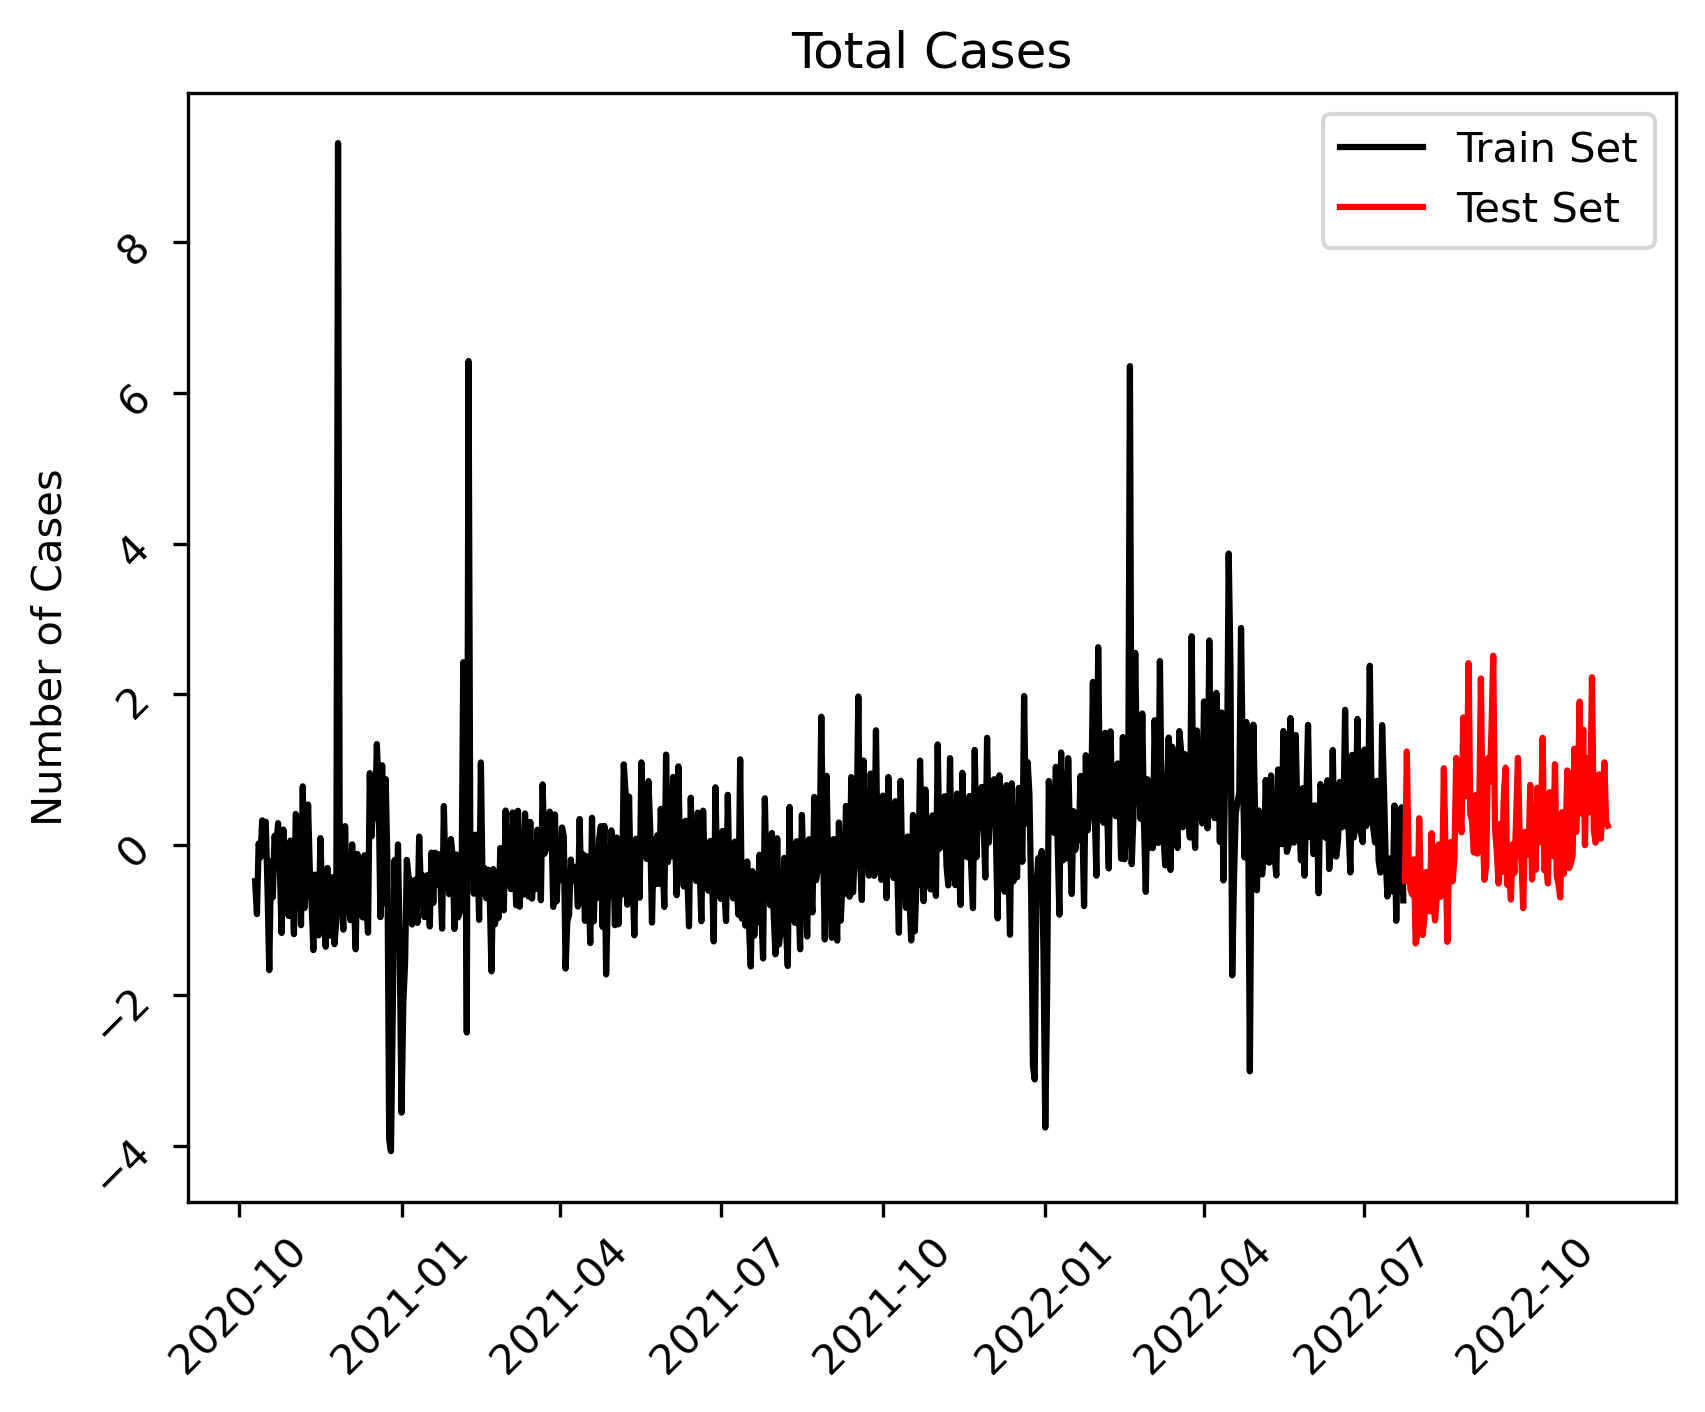
\includegraphics[width=\linewidth]{pics/cases_total_NL.png}
  \caption{The standardized total number of cases between the first of October 2020 and the first of October 2022}
  \label{fig:total cases NL}
\end{minipage}
\begin{minipage}{.5\textwidth}
  \centering
  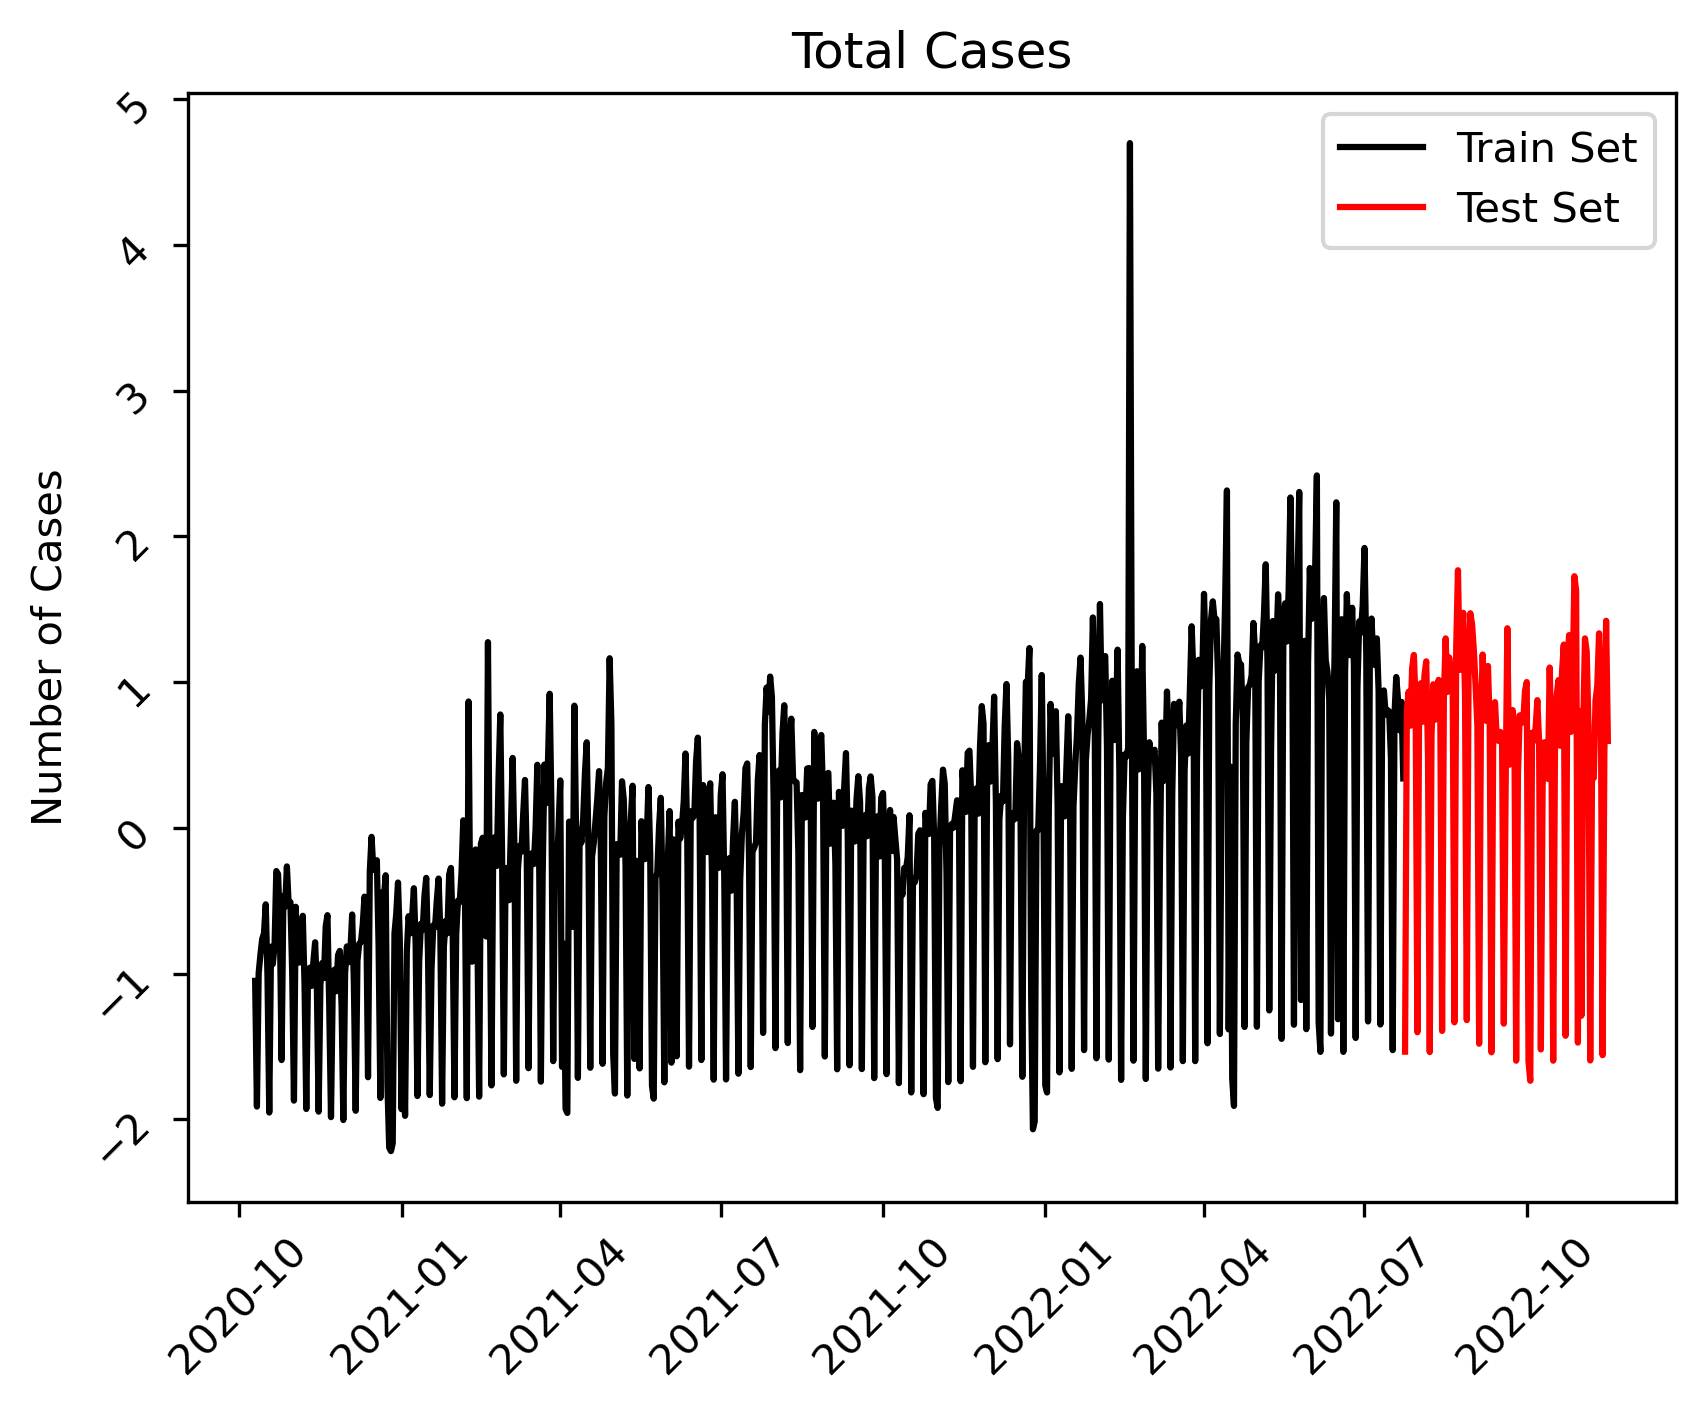
\includegraphics[width=\linewidth]{pics/cases_total_DE.png}
  \caption{The standardized total number of cases between the first of October 2020 and the first of October 2022}
  \label{fig:total cases DE}
\end{minipage}

\begin{minipage}{.5\textwidth}
  \centering
  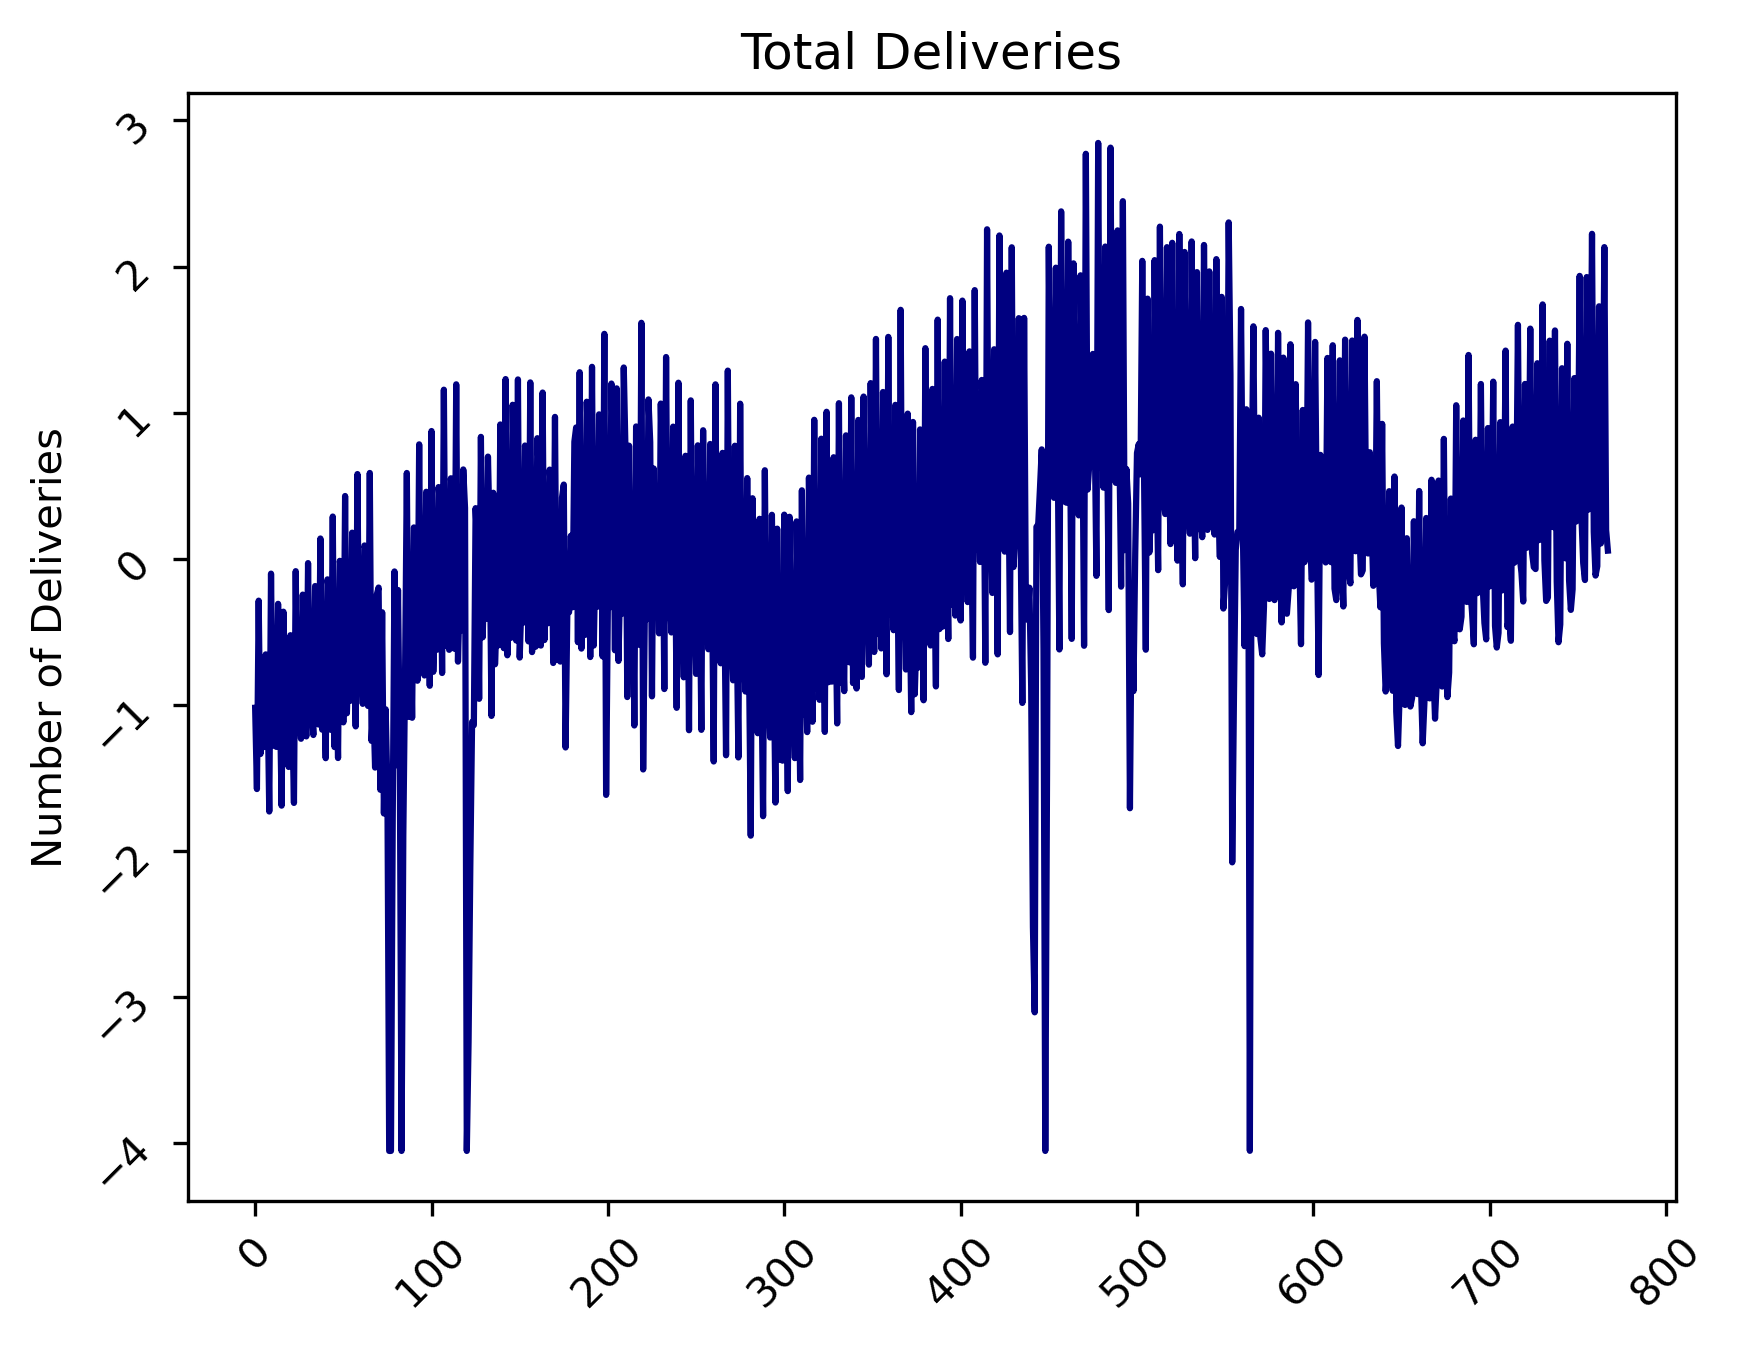
\includegraphics[width=\linewidth]{pics/deliveries_total_NL.png}
  \caption{The standardized total number of NL deliveries between the first of October 2020 and the first of October 2022}
  \label{fig:deliveries_NL}
\end{minipage}
\begin{minipage}{.5\textwidth}
  \centering
  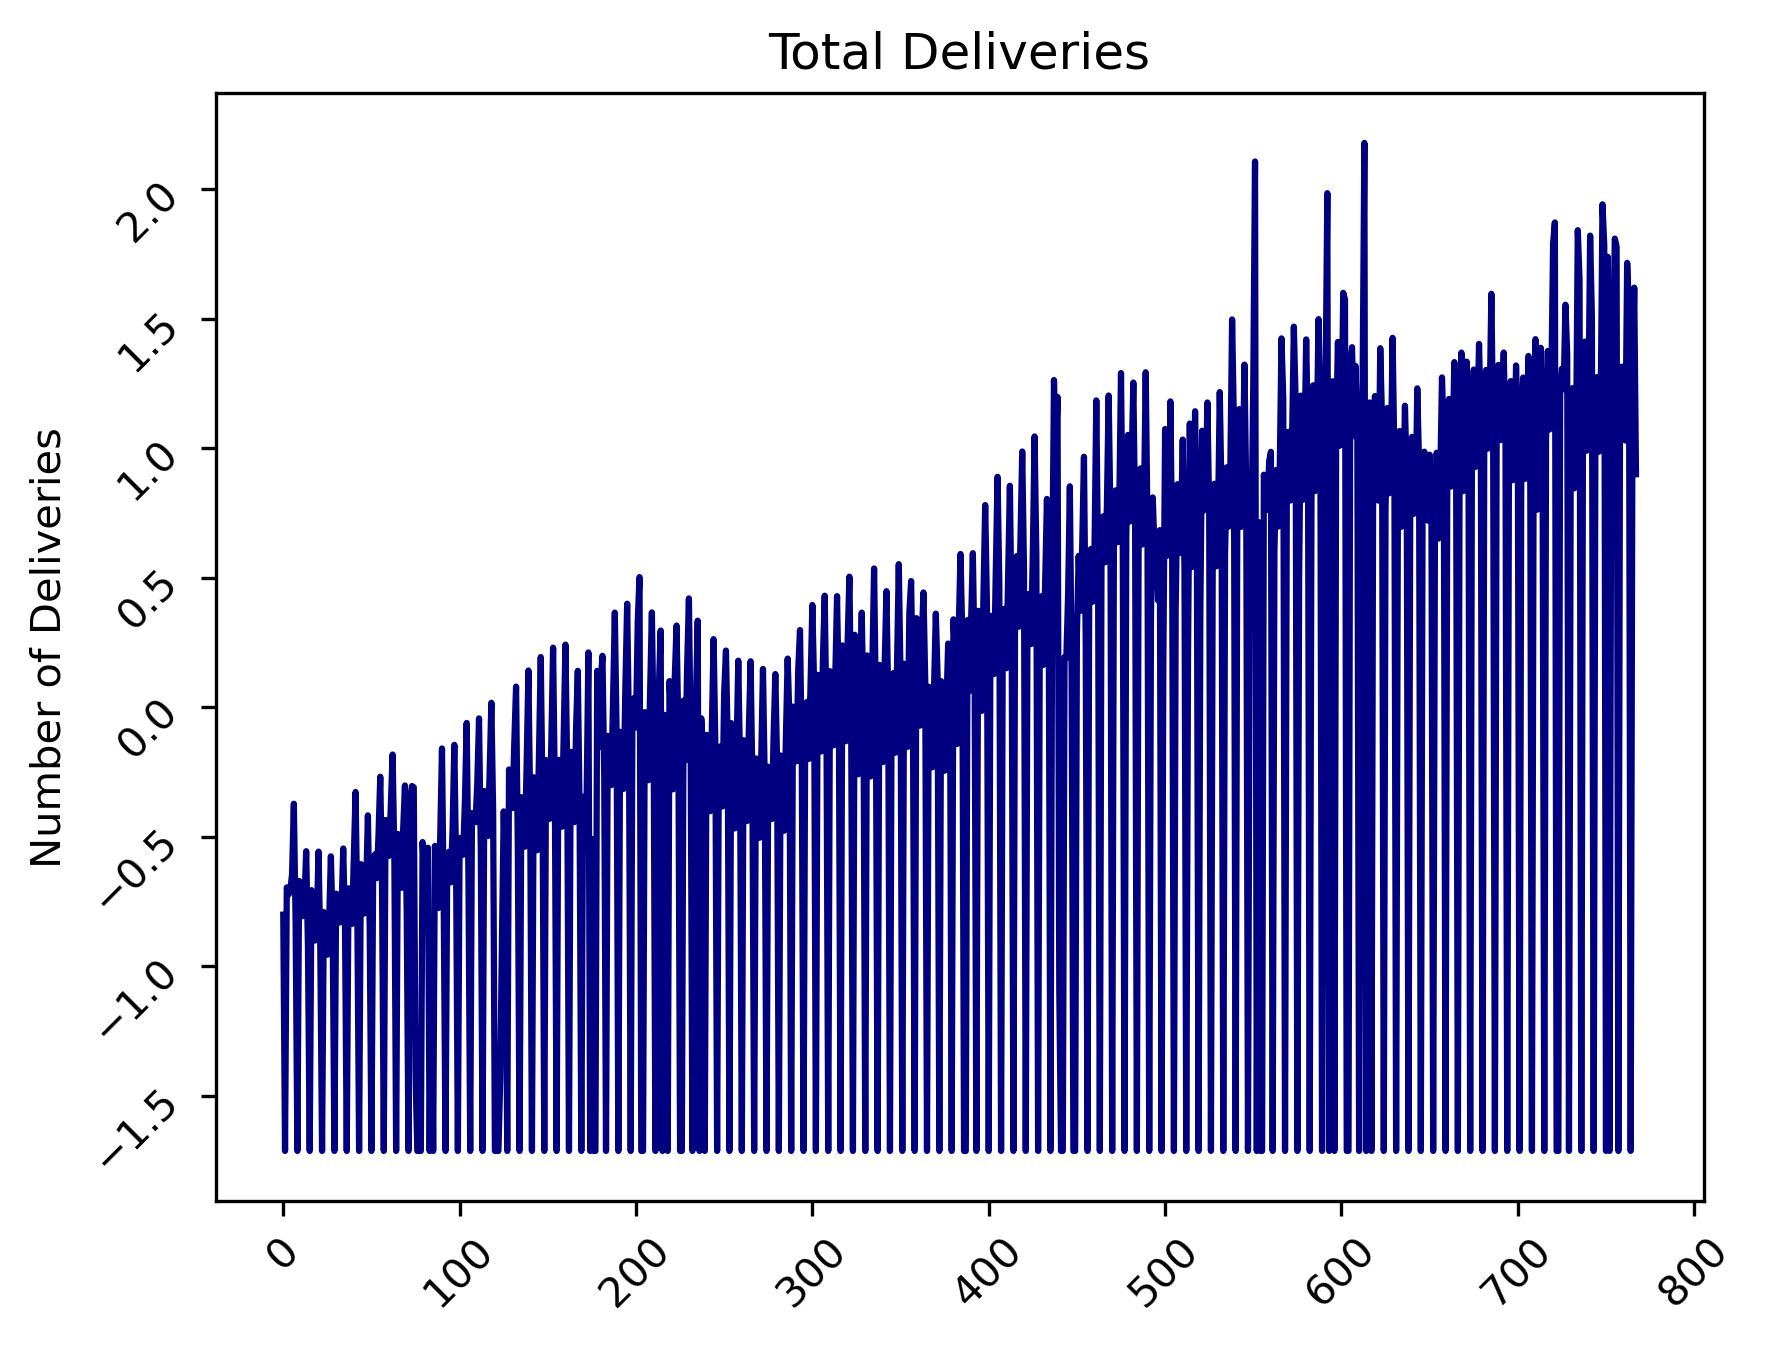
\includegraphics[width=\linewidth]{pics/deliveries_total_DE.png}
  \caption{The standardized total number of NL deliveries between the first of October 2020 and the first of October 2022}
  \label{fig:deliveries_DE}
\end{minipage}

\begin{minipage}{.5\textwidth}
  \centering
  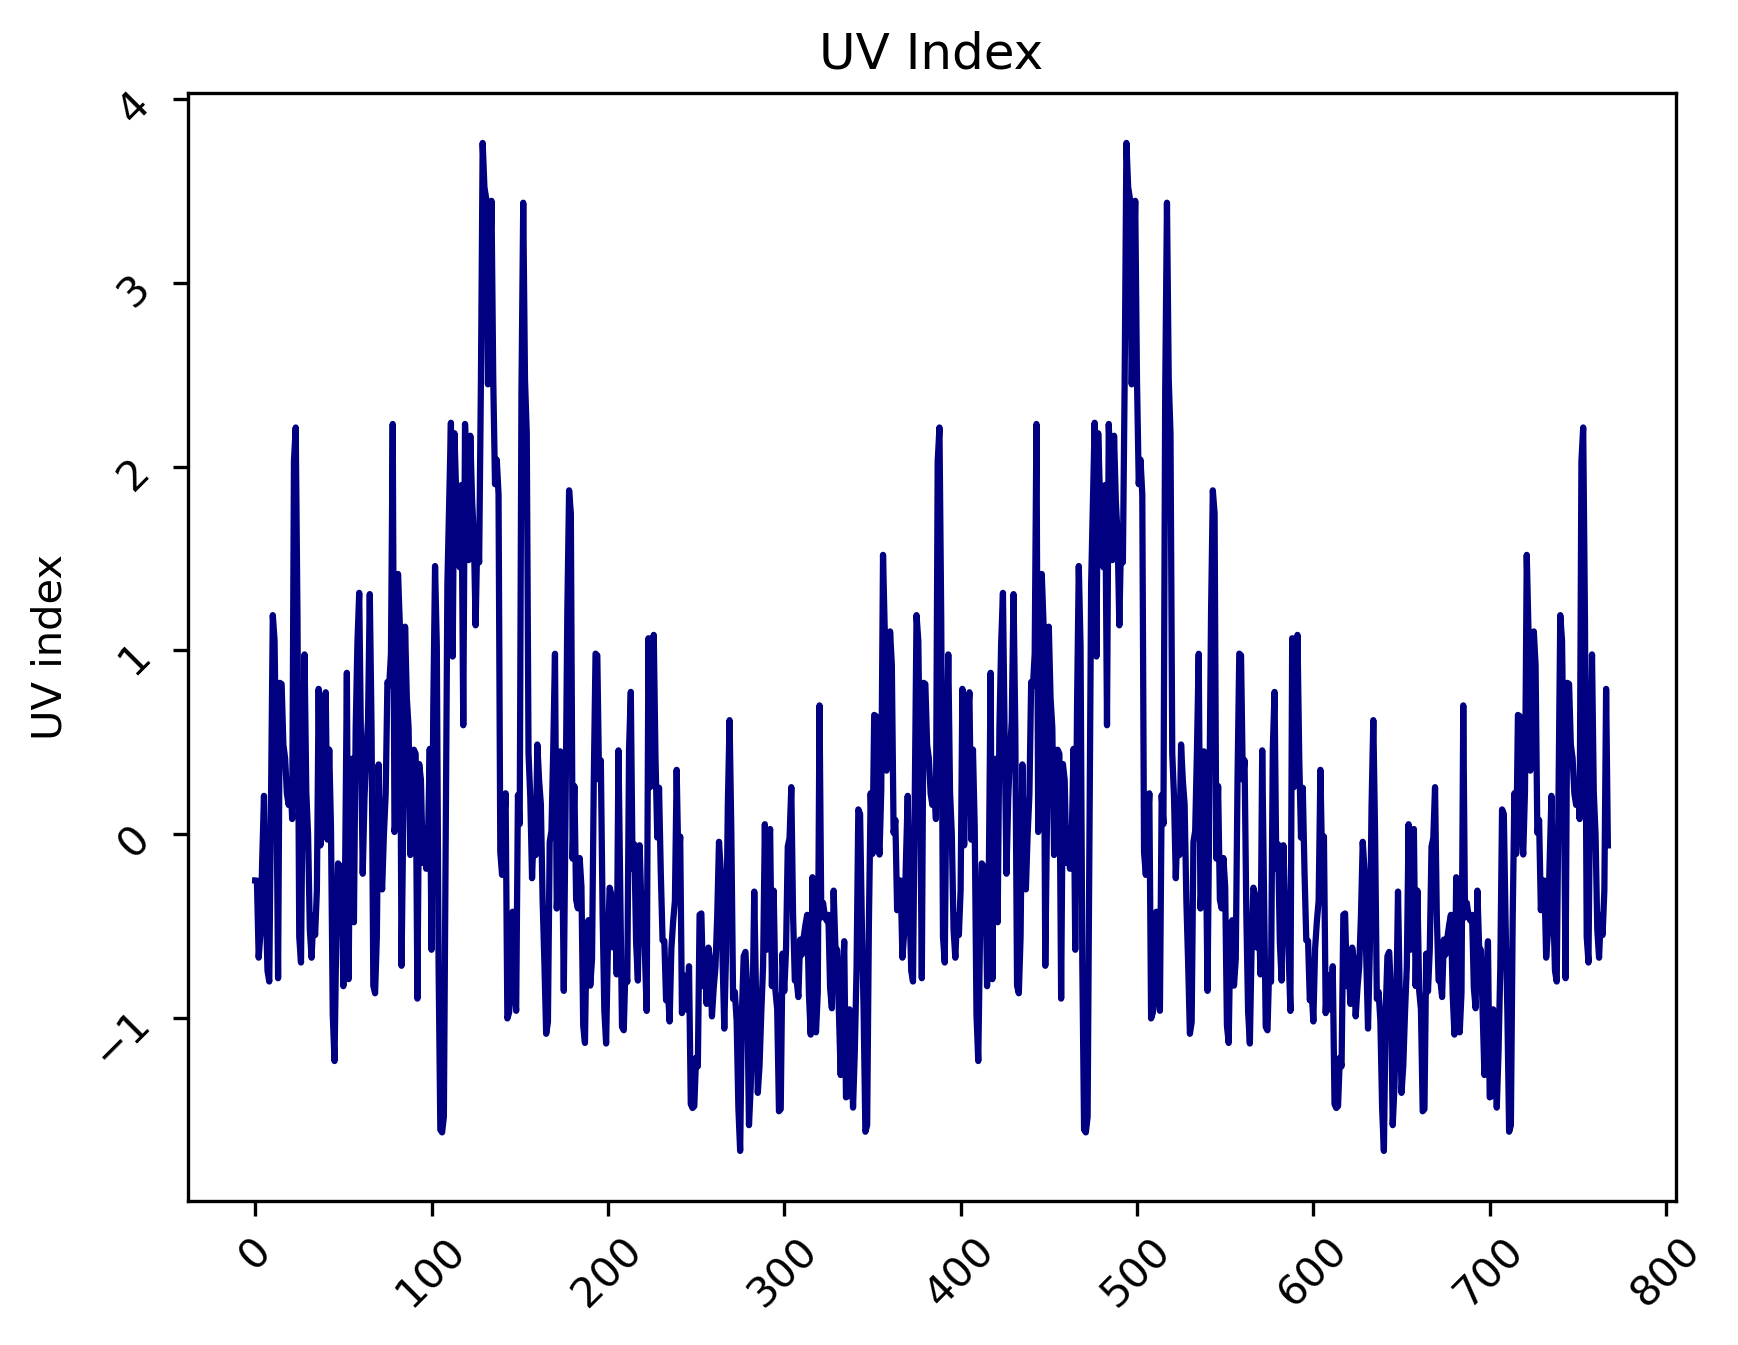
\includegraphics[width=\linewidth]{pics/uv_index_NL.png}
  \caption{The standardized UV index between the first of October 2020 and the first of October 2022}
  \label{fig:UV index NL}
\end{minipage}
\begin{minipage}{.5\textwidth}
  \centering
  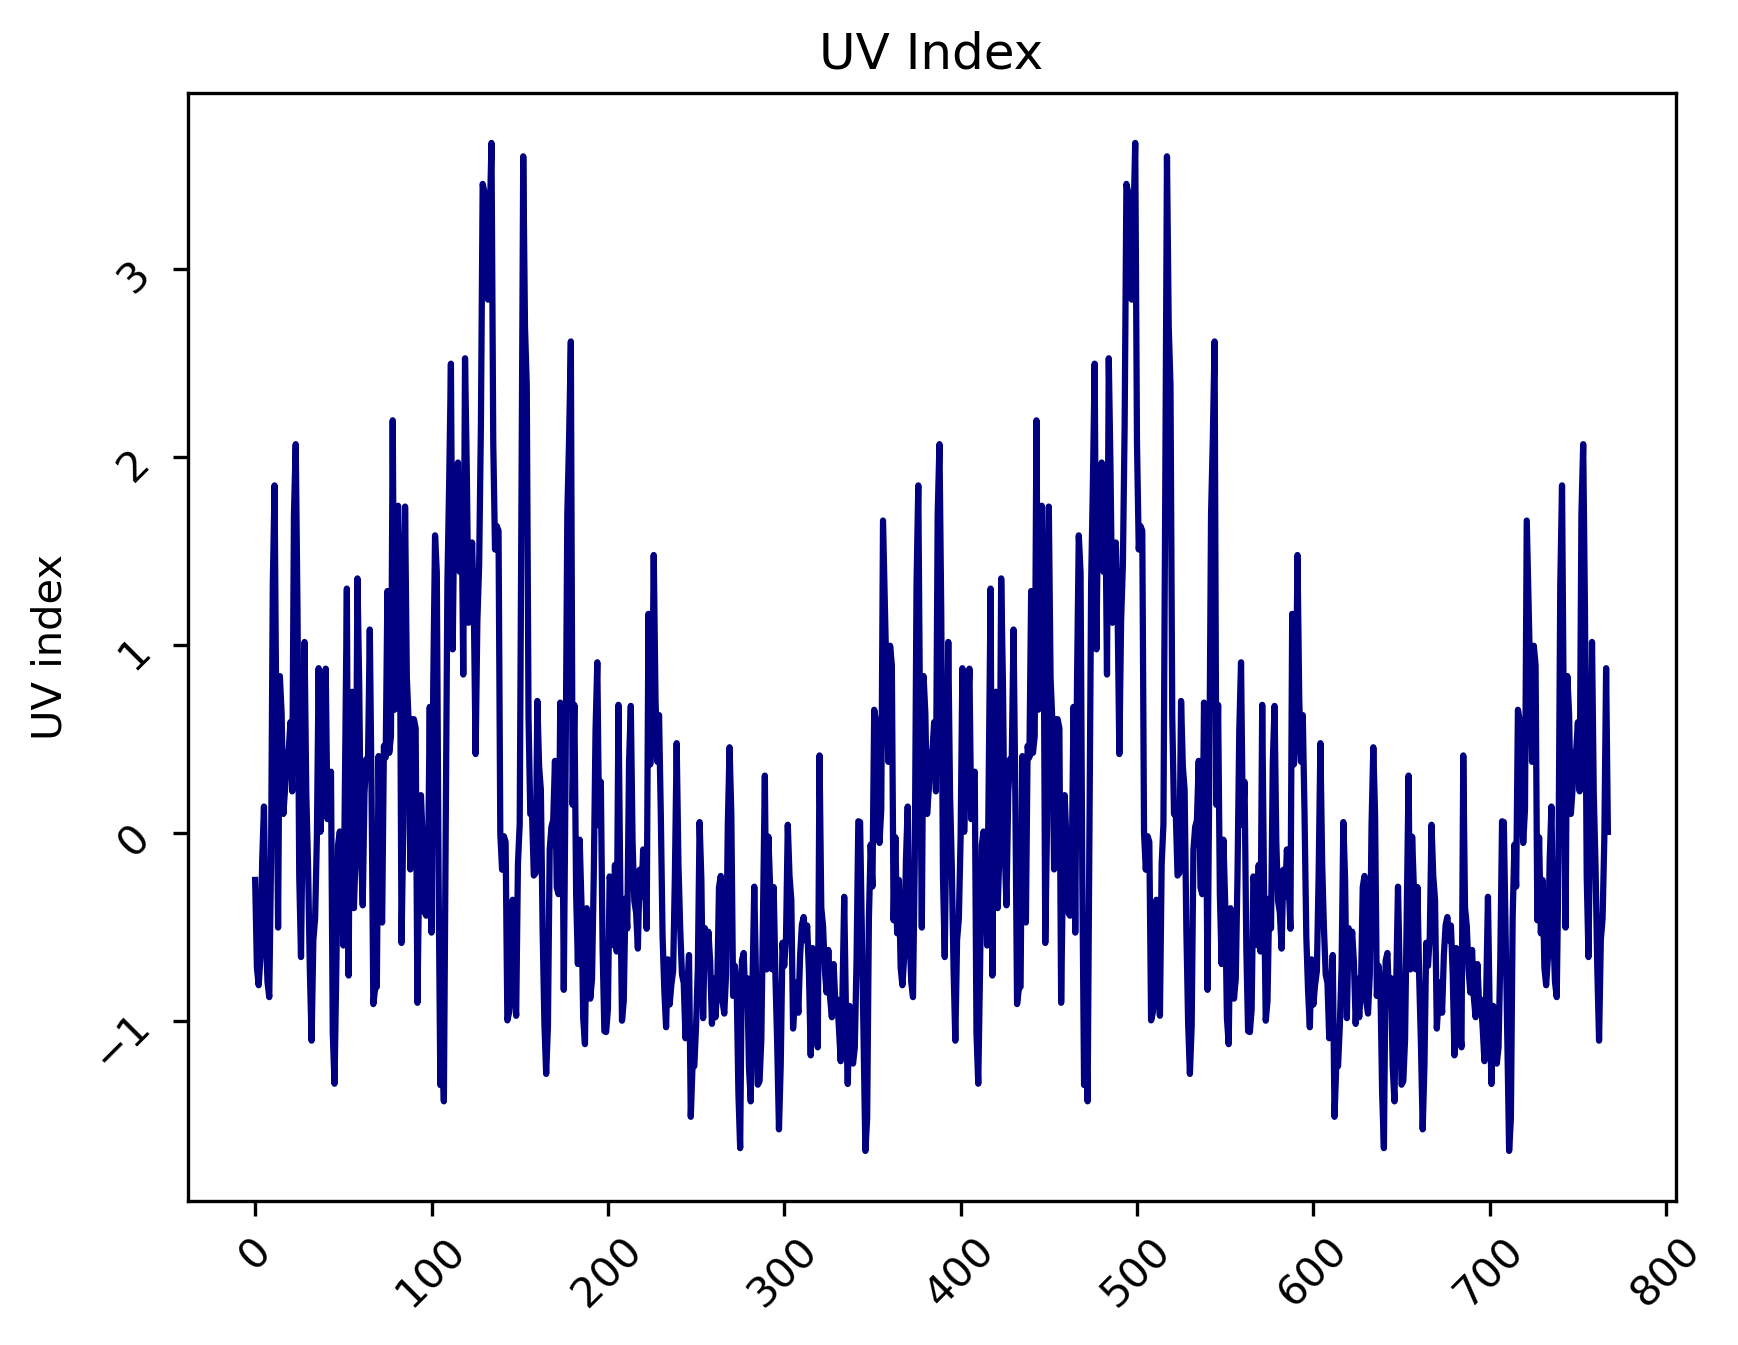
\includegraphics[width=\linewidth]{pics/uv_index_DE.png}
  \caption{The standardized UV index between the first of October 2020 and the first of October 2022}
  \label{fig:UV index DE}
\end{minipage}
\end{figure}

\begin{figure}
\begin{minipage}{.5\textwidth}
  \centering
  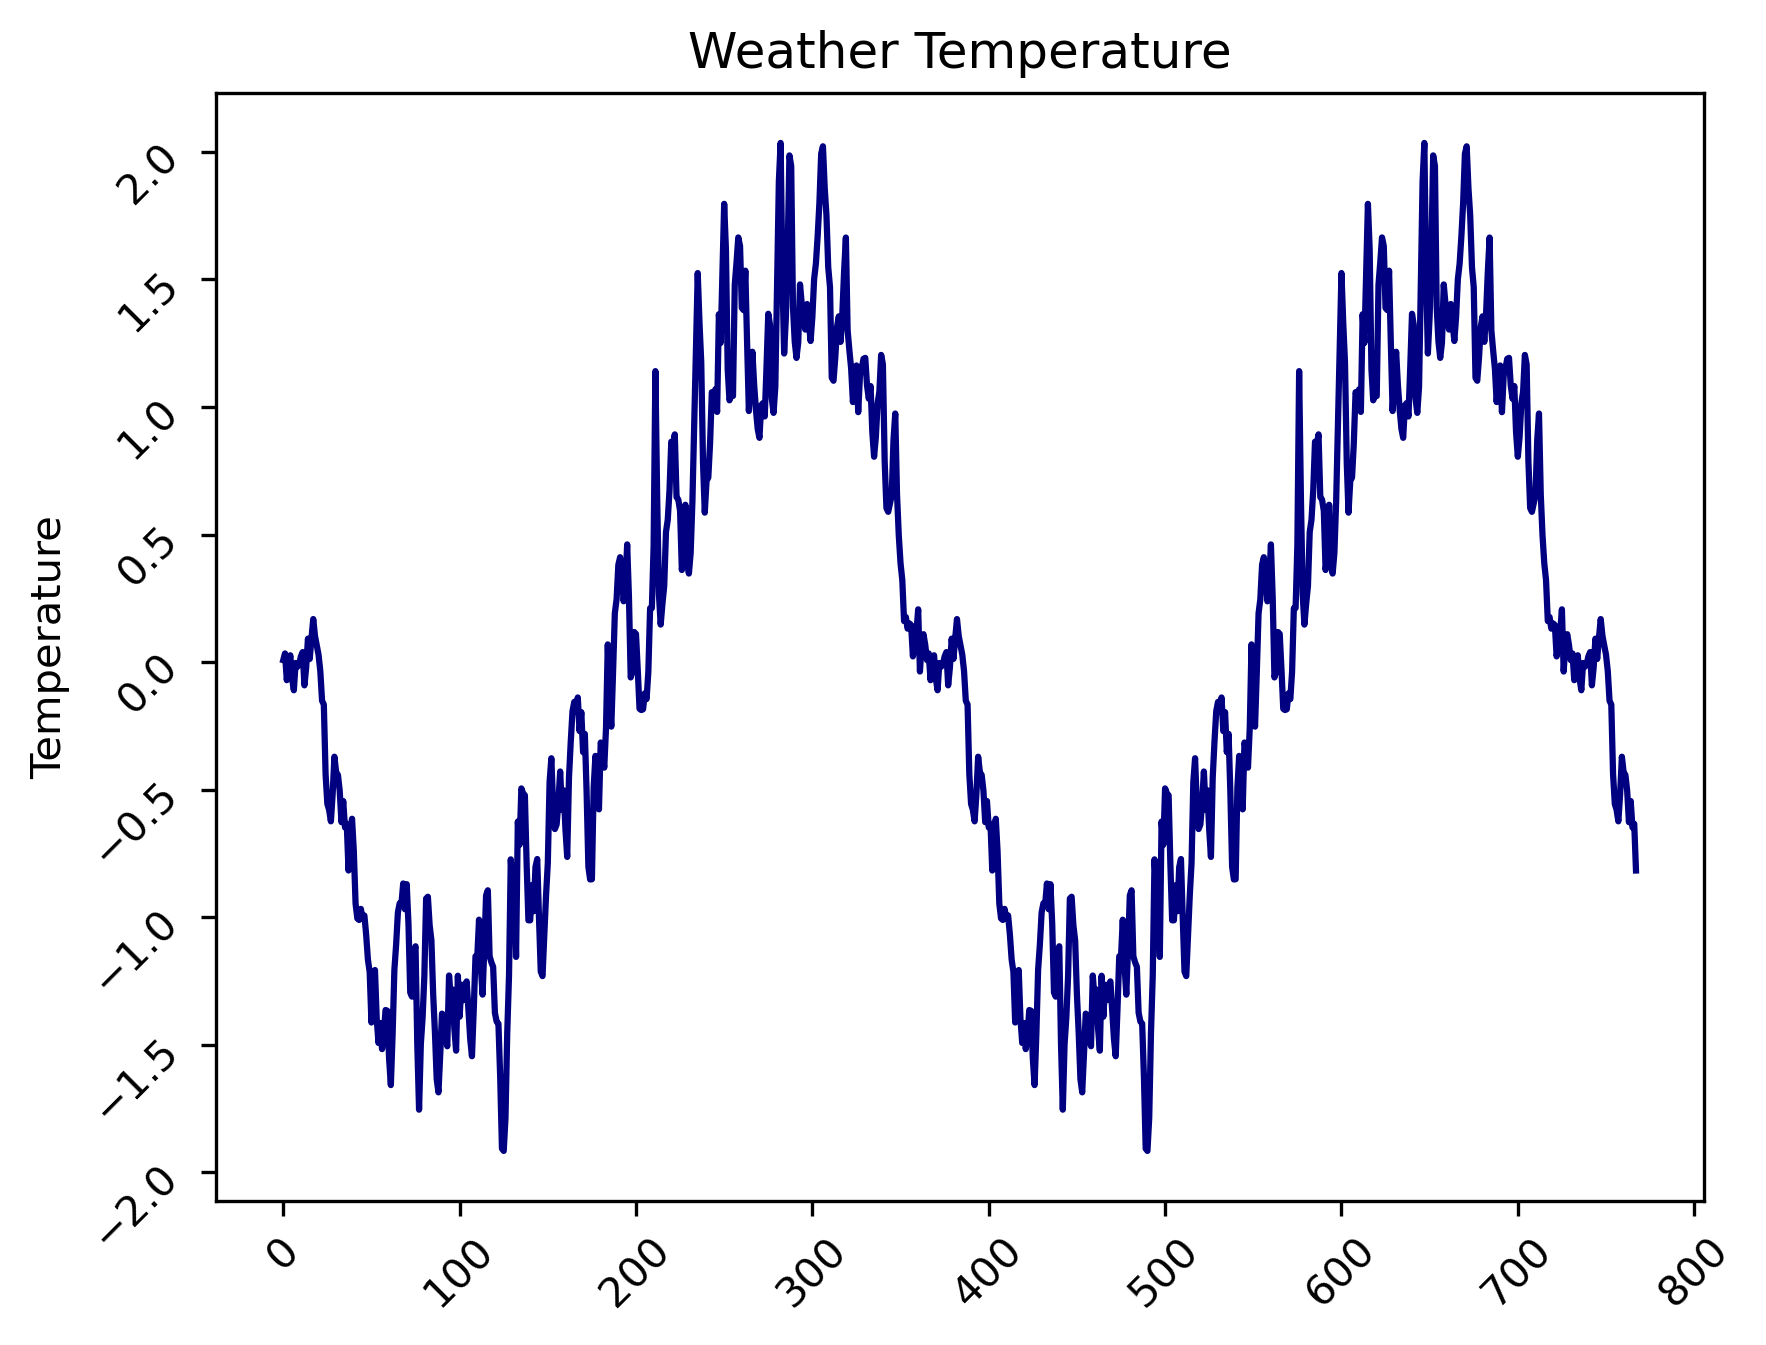
\includegraphics[width=\linewidth]{pics/temperature_total_NL.png}
  \caption{The standardized average temperature in NL between the first of October 2020 and the first of October 2022}
  \label{fig:temperature NL}
\end{minipage}
\begin{minipage}{.5\textwidth}
  \centering
  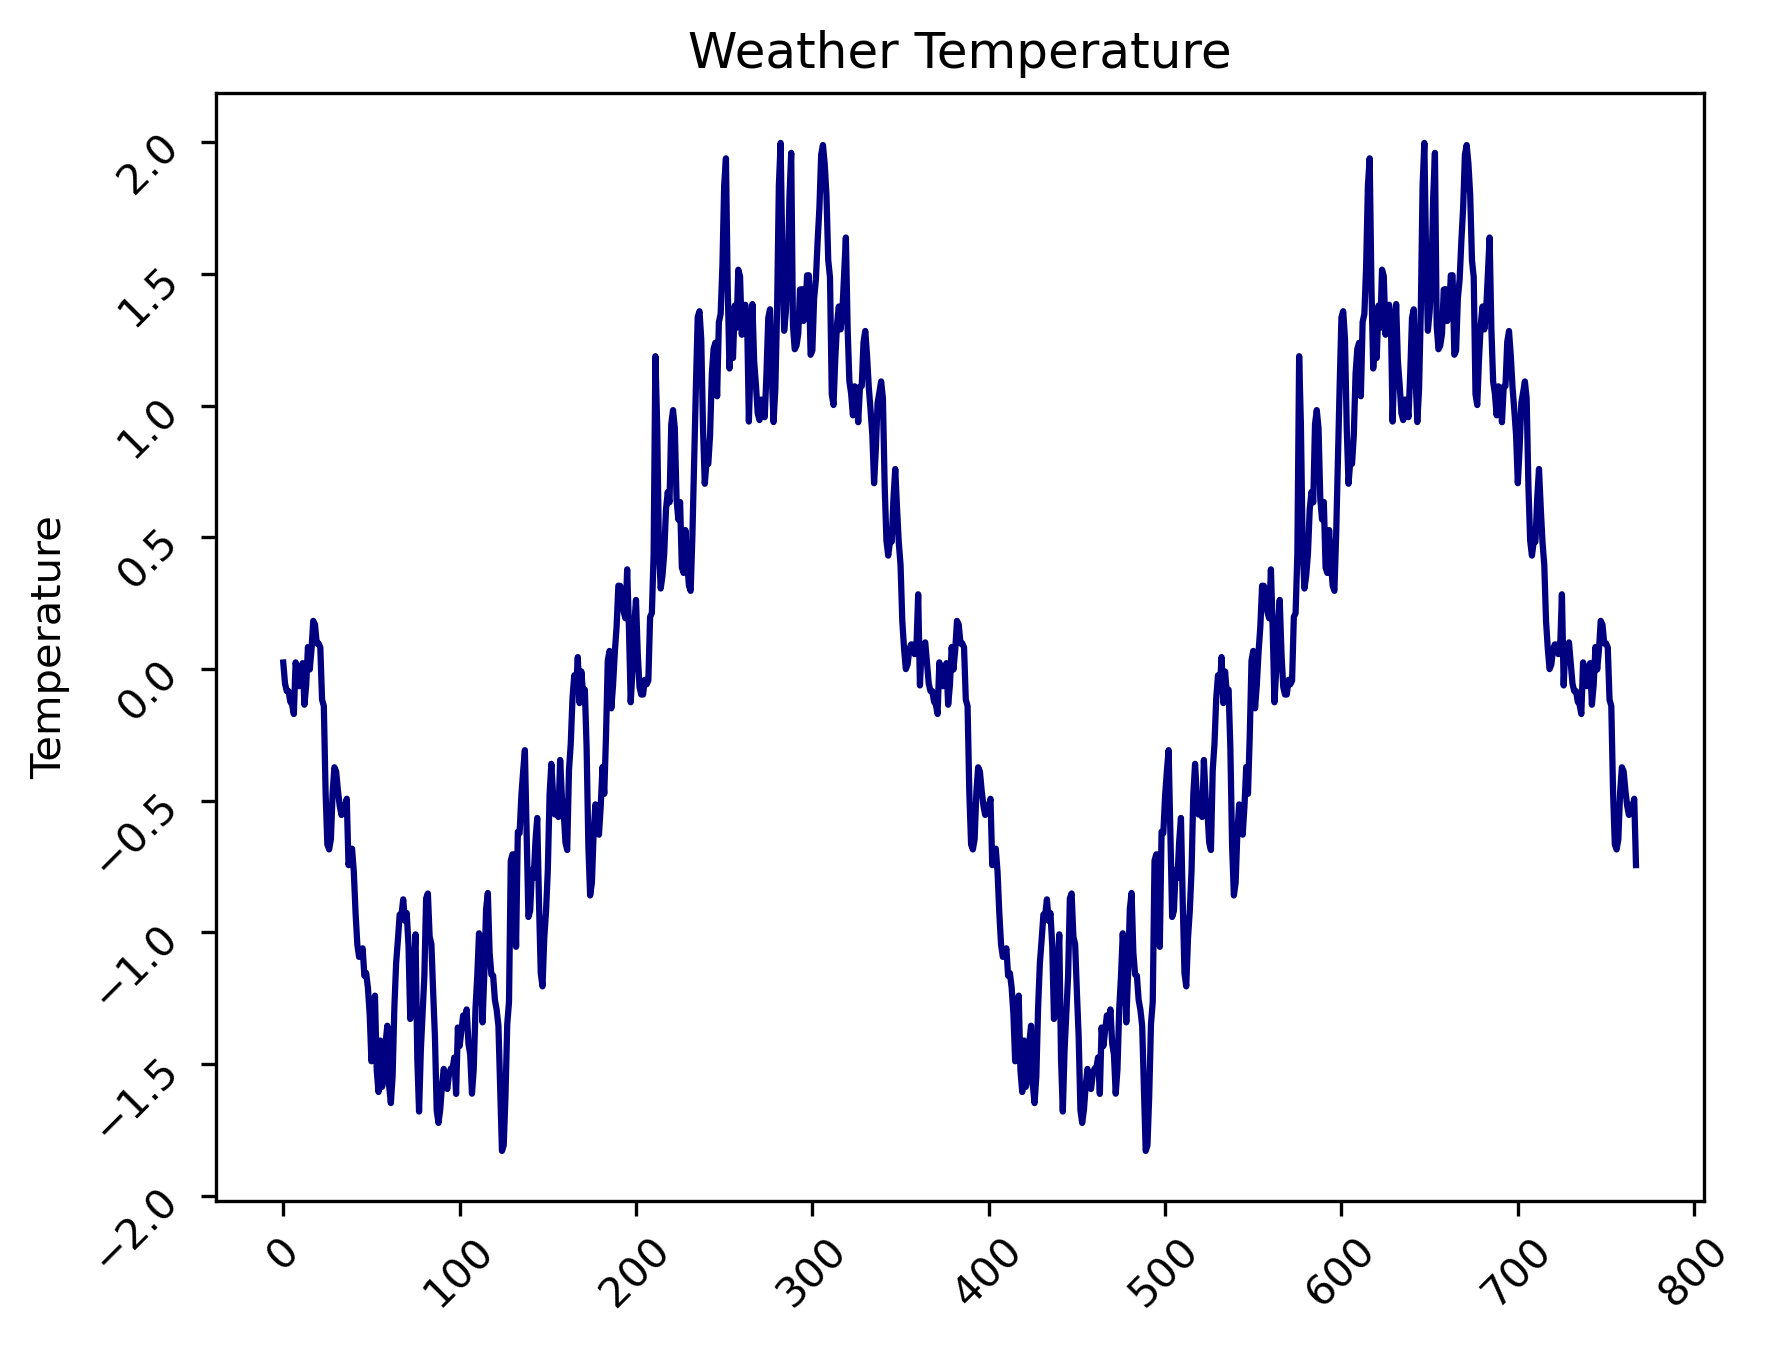
\includegraphics[width=\linewidth]{pics/temperature_total_DE.png}
  \caption{The standardized average temperature in NL between the first of October 2020 and the first of October 2022}
  \label{fig:temperature DE}
\end{minipage}
\end{figure}

As we can see in \autoref{tab:mean_var} the number of cases we want to predict has a high variance. This is expected as cases can come in at random. The high variance with incoming cases has been documented in previous literature \citep{Stolletz2011ArticleManagement}. The continuous numerical variables we want to use are described in table \ref{tab:coninuous_variables_mean_var}. The figured are plotted with the deliveries in \autoref{fig:deliveries_NL} for the Netherlands and \autoref{fig:deliveries_DE} for Germany, the temperature is plotted in \autoref{fig:temperature NL} and in \autoref{fig:temperature DE} for Germany. The feature of the UV index is plotted in \autoref{fig:UV index NL} for the Netherlands and \autoref{fig:UV index DE} for Germany.\\

The choice of dependent variable as the number of cases (Total cases in \autoref{fig:total cases NL} for the Netherlands and in \autoref{fig:total cases DE} for Germany) instead of directly forecasting the workload has to do with a couple of reasons. The number of cases can be closed outside of the system which means the active time does not get recorded. If the workload gets very high, cases get closed in bulk. This means that agents will not spend any time on these cases. This is not a situation that should be taken into account in the data, because we want to predict the total number of cases that come in and should get attention from the agents if there are enough agnets. Another reason not to choose the workload as dependent variable is because there are always people optimising the operations at the customer success team. This means the workload per case can vary a lot and the historic data might not give a good indication on the workload per case in the future.\\

\subsection{Preprocessing}
Because the data is in different orders of magnitude, it is useful to standardize the data. This means that for all the models we will have:
\begin{equation}
    z = \frac{x - \hat{\mu}}{\hat{\sigma}}
\end{equation}
Where $\hat{\mu}$ is the sample mean of the data and $\hat{\sigma}$ is the sample standard deviation of the data. $\hat{\mu}$ and $\hat{\sigma}$ are saved such that it is possible to scale the data back in exactly the same way.\\

For the models, ARIMA, ARIMAX and VARIMAX models, it is important to take a look at order of integration I and for the lag selection it is important to look at the autocorrelation (Figures \ref{fig:autocorrelation NL} and \ref{fig:autocorrelation DE}) and the partial autocorrelation (Figures \ref{fig:partial autocorrelation NL} and \ref{fig:partial autocorrelation DE}). In \autoref{tab:dicktest} the p-values of the Engle-Granger cointegration test are displayed \citep{Engle1987Co-IntegrationTesting}. The Engle-Granger test has a null hypothesis of cointegration between Y and the first lag of Y. In \autoref{tab:dicktest} the p-values show that with a 5\% significance level we cannot say the data is not cointegrated if the order of differencing is 0 in both the Netherlands and Germany. If we difference the data 1 time, we can say with a significance level of less than 1\% that the data is not cointegrated. The same can be said if we difference the data two or three times. For the ARIMA models we will difference the data once since there is no advantage in continuing differencing if the data is not cointegrated and differencing the data has the disadvantage of becoming less easy to interpret and with every time the data is differenced, you lose 1 data point.\\
\begin{table}[]
    \centering
    \begin{tabular}{|c|c c|}\hline    
        Difference & Netherlands & Germany\\ \hline
        0 & 0.4905  & 0.0921 \\
        1 & 0.0 & 0.0 \\
        2 & 0.0 & 0.0 \\
        3 & 0.0 & 0.0 \\
        4 & 0.0 & 0.0 \\
    \hline 
    \end{tabular}
    \caption{P-values of the augmented Dickey Fuller test for stationarity on total number of cases}
    \label{tab:dicktest}
\end{table}

\begin{figure}
\begin{minipage}{.5\textwidth}
    \centering
    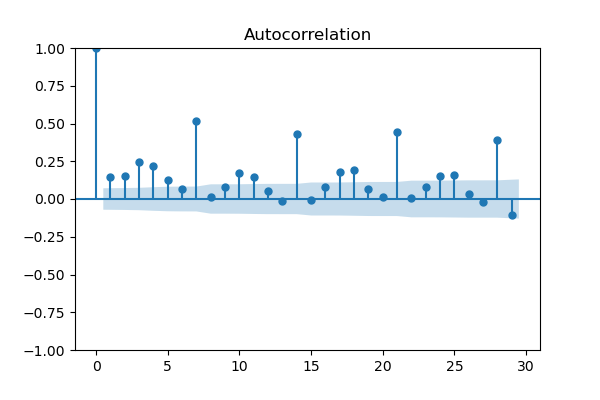
\includegraphics[width=\linewidth]{pics/acf_1_diff_NL.png}
    \caption{Autocorrelation plot of first differenced data in the Netherlands}
    \label{fig:autocorrelation NL}
\end{minipage}
\begin{minipage}{.5\textwidth} 
    \centering
    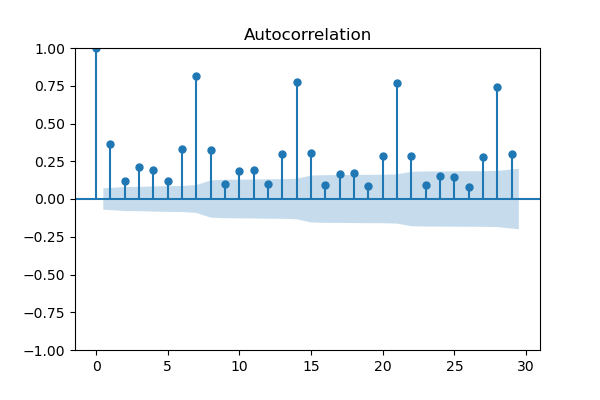
\includegraphics[width=\linewidth]{pics/acf_1_diff_DE.png}
    \caption{Autocorrelation plot of first differenced data in Germany}
    \label{fig:autocorrelation DE}
\end{minipage}
\end{figure}
\begin{figure}
\begin{minipage}{.5\textwidth}
    \centering
    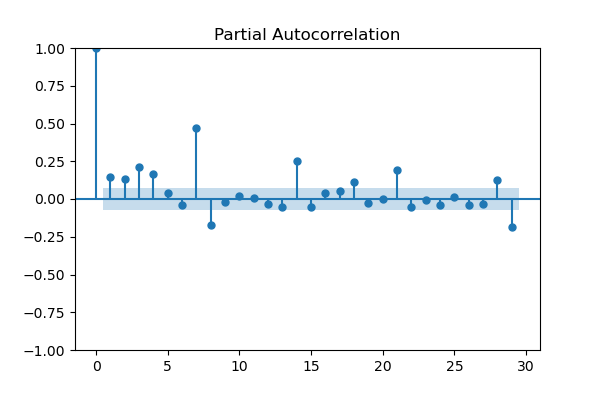
\includegraphics[width=\linewidth]{pics/pacf_1_diff_NL.png}
    \caption{Partial Autocorrelation plot of first differenced data in the Netherlands}
    \label{fig:partial autocorrelation NL}
\end{minipage}
\begin{minipage}{.5\textwidth} 
    \centering
    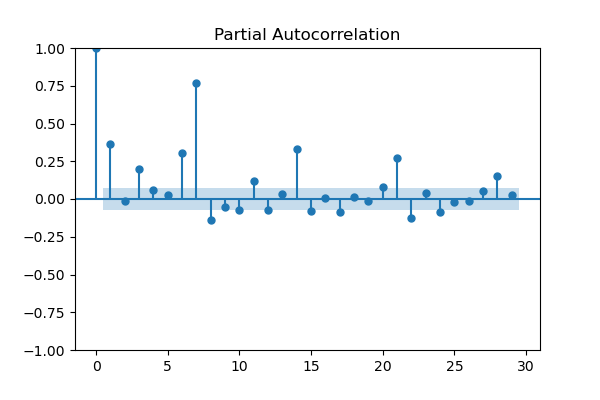
\includegraphics[width=\linewidth]{pics/pacf_1_diff_DE.png}
    \caption{Partial autocorrelation plot of first differenced data in Germany}
    \label{fig:partial autocorrelation DE}
\end{minipage}
\end{figure}